\documentclass[12pt]{article}
\usepackage[breaklinks=true]{hyperref}
\usepackage[margin=0.75in]{geometry}

\usepackage{graphicx}
\usepackage{color}
\usepackage{amsmath}

\definecolor{pblue}{rgb}{0.13,0.13,1}
\definecolor{pgreen}{rgb}{0,0.5,0}
\definecolor{pred}{rgb}{0.9,0,0}
\definecolor{pgrey}{rgb}{0.46,0.45,0.48}

\usepackage{listings}
\lstset{language=Java,
  showspaces=false,
  showtabs=false,
  tabsize=2,
  breaklines=true,
  showstringspaces=false,
  breakatwhitespace=true,
  commentstyle=\color{pgreen},
  keywordstyle=\color{pblue},
  stringstyle=\color{pred},
  basicstyle=\ttfamily,
  frame=single,
  moredelim=[il][\textcolor{pgrey}]{$$},
  moredelim=[is][\textcolor{pgrey}]{\%\%}{\%\%}
}

\title{Concurrency: Writing Multithreaded Programs in Java}
\author{
	Melvyn Ian Drag
}
\date{\today}


\begin{document}
\maketitle

\begin{abstract}
Up until now we've written \textbf{serial} code. Today we will learn to write
\textbf{concurrent} code. In other words, before we only programmed our machines
to do one thing at a time. Now we will write programs that multitask - or at
least give the illusion of multitasking.
\end{abstract}

\section{Introduction}
Concurrency seems like a simple concept - you can program a computer to do
several things at once. If your computer is using a multicore processor like an
intel-iX then it's very easy to image a computer doing simultaneous/concurrent
operations, because there are acutally multiple CPU cores working at once. But
even single cores can give the illusion of doing things concurrently! You will
learn about how all our fancy modern operating systems like Windows and Linux
and MacOS do this via ``Context Switching".

Nevertheless, the business of actually \textit{programming} your computer to do
things concurrently is quite challenging and takes years of thought and
disciplined practice to do correctly. Don't take my word for it, take
\textit{Enrique Lopez Manas'} (some google developer I found on medium.com) word
for it:

\textit{Multithreading is an entire discipline that takes years to master and
properly understand. We will keep a short introduction in this article}

Link:
\url{https://medium.com/google-developer-experts/on-properly-using-volatile-and-synchronized-702fc05faac2}

As he said in the intro to the article linked above - we too will keep our intro
short and sweet. The purpose of this lecture is to get your ``toes in the water"
so to speak, and then you can go on the internet and research more about
concurrent programming in Java. 

\subsection{What we'll learn tonight}
We are going to learn about:
\begin{enumerate}
\item Threads
\item Runnables
\item synchronized statements
\item synchronized functions
\item Atomic variables
\item Take another look at primitives
\end{enumerate}

\section{Get the Class Repo}
Make sure to download the latest iteration of the class repository so you can
get all the code we are going to be using. You could download the files one by
one throughout the night, but it is easier to just download everything.

\section{The problem of the Night}
\label{problemStatement}

\begin{center}
\textbf{A reduce operation}
\end{center}

A reduce operation is one where you take a big list of values and reduce them
down to a single value. A common reduce operation is to sum all the numbers in a
List. Another is to find the largest value in a  List. Or the smallest. Or
multiply all the numbers.

Tonight we will focus on the sum operation. You should already know how to do
this serially - that is, with one thread.

Here is the code you might come up with:

\lstinputlisting{MyCode/SerialSum/SerialSum.java}

And here are the results of running the code with various inputs. Compare your
machine's performance to mine to see how it compares to a T450 with an i5
processor and 8GB ram.

\begin{figure}[h]
  \label{serialresults}
  \centering
    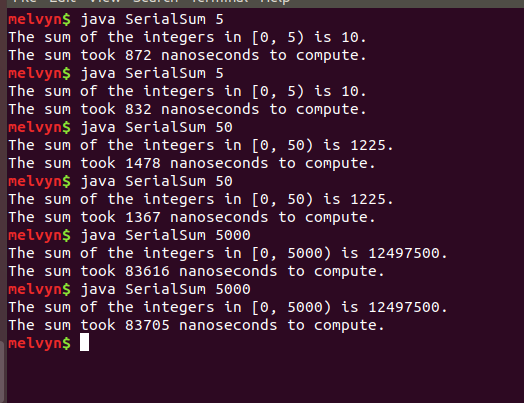
\includegraphics[width=0.5\textwidth]{Images/SerialResults.png}
  \caption{Testing summing numbers from 0 to 4, 49, 4999.}
\end{figure}

And we can quickly verify that this silly little computation is correct by using
a little trick from math class:

\begin{equation}
\label{sumformula}
	\sum_{i=0}^{N-1}i = \frac{(N-1)*N}{2}
\end{equation}

And so, according to equation \ref{sumformula}, we can compute the sums we just
tested in Java.

\begin{align*}
	\sum_{i=0}^{4}i &= \frac{(4)*5}{2} \\
					&= 10 \\
	\sum_{i=0}^{49}i &= \frac{(49)*50}{2} \\
					 &= 1225 \\
	\sum_{i=0}^{4999}i &= \frac{(4999)*5000}{2} \\
					&= 12497500
\end{align*}

Look at figure \ref{serialresults} and compare the outputs there to the values
we computed with our little math trick. We should all now agree that our simple
SerialSum.java is working correctly - but can we make it \textit{faster}? Of
course we can, that's the purpose of tonight's lecture!

\section{Threads}
To do concurrent things, Java uses \textbf{Threads}. So far our code has been
single-threaded ( aka `serial' ). Multithreaded applications, like we will write
now, are referred to synonymously as `concurrent' programs.

\subsection{Create Threads by Subclassing \textit{Thread}}

Note that the our simple class \textit{SubclassThread} contains a \textit{run()}
method. Do not call that method. That is the function that is called when you
call \textit{.start()}. 


\begin{center}
{\Large\textbf{Attention!}}

\textbf{Read the abvove and the code sample
carefully. You DO NOT call the run() method yourself. That function is called
when you call .start().}
\end{center}

\lstinputlisting{MyCode/SubclassThread/SubclassThread.java}

\begin{figure}[ht]
  \label{runningSubclassThread}
  \centering
    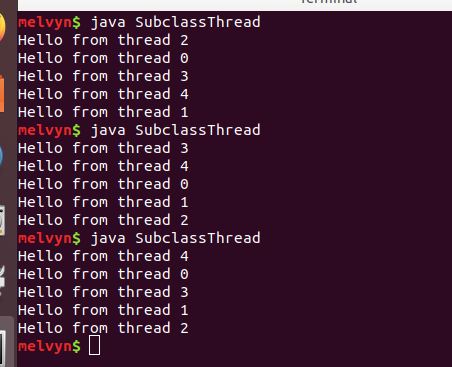
\includegraphics[width=0.5\textwidth]{Images/runningSubclassThread.png}
  \caption{Creating a class that extends `Thread'}
\end{figure}


Note that the order in which the threads execute the \textit{run()} method is
non-deterministic. Each run, they execute in a different order. This is
something to be aware of. For today's lecture it doesn't matter, but for other
code you write you will have to be careful because of this. Refer to image
\ref{runningSubclassThread} to see this code in action.

\subsection{Create Runnables by Subclassing \textit{Runnable}}

Whereas \textit{Thread} is a class, \textit{Runnable} is an interface. When you
do the homework, you will read about the relative merits of using the class vs
the interface. For now, we are just going to write a could of simple examples
and use them.

Note that the class that implements \textit{Runnable} still has to define a
\textit{run()} method. Just as with the \textit{Thread} class, when we call
\textit{.start()}, the \textit{run()} method is called.


\lstinputlisting{MyCode/SubclassRunnable/SubclassRunnable.java}

\begin{figure}[ht]
  \label{runningSubclassRunnable}
  \centering
    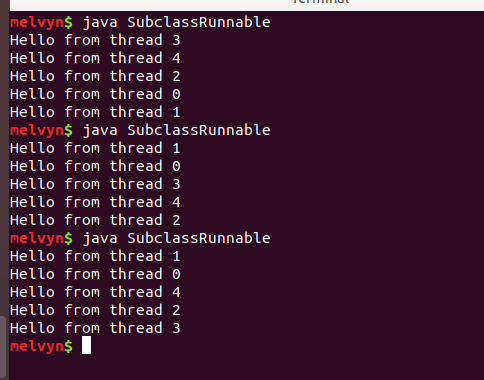
\includegraphics[width=0.5\textwidth]{Images/runningSubclassRunnable.png}
  \caption{Creating a class that extends `Runnable'}
\end{figure}


Note that the order in which the threads execute the \textit{run()} method is
non-deterministic. Each run, they execute in a different order. This is
something to be aware of. For today's lecture it doesn't matter, but for other
code you write you will have to be careful because of this. Refer to image
\ref{runningSubclassRunnable} to see this code in action.


\subsection{You need to read more}
I am confident discussing this topic because I've read a stack of references. To
cement your knowledge of what I've just said about threads, and about what I am
about to say, you 100\% should read the official Java tutorial about threads.

It is here:

\url{https://docs.oracle.com/javase/tutorial/essential/concurrency/}

After today's lecture, this material should be digestible.

\section{The \textit{synchronized} keyword}

I've already told you - mastering concurrency takes time. You need to learn
about many errors that could arise and learn how to mitigate them. There is no
time to address them all, so I'll present a basic one to you. This is a very
intellectually rewarding ( and financially if you can master the topic and get a
job doing it ) topic.


A major problem when writing concurrent code is ensuring that two competing
thread don't access computer memory at the same time. If you are in class and
reading this, make sure to ask me to draw a picture on the board to illustrate
the problem of competing memory accesses.

{\LARGE Draw a diagram showing that two threads accessing the same memory
location without syncronization can cause mistakes in your code. This is one of
the most common and insidious problems you come across}

\subsection{The example of the day in code}

For the heck of it I chose to implement this example by implementing the
Runnable interface. You can tinker with this code and make it use the Thread
base class. That would be a fun project for you. In general, this code is the
same as our SerialSum example, except it uses a few threads to do the work
instead of just one.

\lstinputlisting{MyCode/IntSynchronized/SynchronizedSumReduce.java}

\subsection{A Problem! And a Solution! Use the Right Datatype}
Note that an issue with this is if we try to run the code with parameter
\textit{1000000}. The \textit{int} datatype cannot hold the sum of 0 to 999999,
and overflows. Try to run the code and you will see the solution.

Change the \textit{partialSum} and \textit{total} variables to be \textit{long}s
instead of \textit{int}s and then they can hold larger values.

See \textit{MyCode/LongSynchronized/SynchronizedSumReduce.java}. 

Of course this isn't a 100\% solution - the long data type can also be
overflowed! Java has classes to handle data that is larger than the 8 bytes of a
long. I believe the big number classes are called \textit{BigInt} or
\textit{BigNum} or \textit{BigInteger} or the like.

{\Large Exercise: Have class find the name of the classes for integers larger
than 8 bytes in Java}

We aren't going to use those today, but they are super simple classes to use,
if you want to goof around with them just look through the docs you find online
and write some toy examples.


\subsection{Forgetting to synchronize my threads caused an error!}

Look at this code and note that the \textit{updateTotal} method is not
synchronized. Then look at the output of the code shown in figure
\ref{raceCondition}  and note that the output is wrong. The right output can
computed using the formulas given in section \ref{problemStatement}

The code is in \textit{MyCode/RaceConditions/NonSynchronizedSumReduce.java} This
code is the same as the code in the \textit{SynchronizedSumReduce} example,
except the \textit{update} method was changed from this:

\begin{lstlisting}
private synchronized void updateTotal( int partialSum ){
	total += partialSum;
}
\end{lstlisting}

to this:

\begin{lstlisting}
private void updateTotal( int partialSum ){
	try{ Thread.sleep(10);}
	catch(Exception e){}
	total += partialSum;
}
\end{lstlisting}

Refer to figure \ref{raceCondition} to see that the output now changes each run,
because the threads are making memory accesses in a non synchronized manner.

Note to self - these notes need an image of race conditions. If you are reading
them and are confused by race conditions, don't hesitate to contact me so I can
explain it.

\begin{figure}[ht]
  \label{raceCondition}
  \centering
    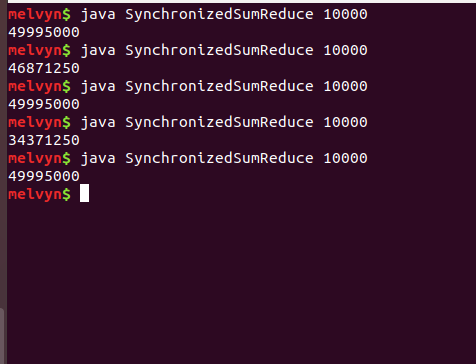
\includegraphics[width=0.5\textwidth]{Images/raceCondition.png}
  \caption{Creating a class that extends `Runnable'}
\end{figure}

{\Large\textbf{Take away: Whenever multiple threads are accessing some shared
memory - in this case they are all accessing the shared ( static ) variable
`total' - make sure to  synchronize their accesses.}}

\section{Break and Experiment. 15 minutes.}
Take some time now to experiment with what I have said. Note that I added a
sleep to the raceCondition example. Try adding that sleep to the properly
working example and notice that it doesn't affect the results. By doing this you
will gain some good insight.

\section{ Another interesting thing - 10 minutes }
Look at my race condtion code. Note that I have broken up the sum computation
into 4 worker threads. Each thread gets a slice of the total sum to compute.
Here is the chunk of the ArrayList given to each thread:

\begin{lstlisting}
List<Integer> intList1 = intList.subList(0, N/4); // upperBound is Exclusive
List<Integer> intList2 = intList.subList(N/4, N/2); // lowerBound is inclusive
List<Integer> intList3 = intList.subList(N/2, 3*N/4); // lowerBound is inclusive
List<Integer> intList4 = intList.subList(3*N/4, N); // lowerBound is inclusive
Thread t1 = new Thread(new SynchronizedSumReduce(intList1));	
Thread t2 = new Thread(new SynchronizedSumReduce(intList2));
Thread t3 = new Thread(new SynchronizedSumReduce(intList3));
Thread t4 = new Thread(new SynchronizedSumReduce(intList4));
\end{lstlisting}

This didn't come from thin air - this is from the RaceCondition example.Note
that in the image that shows the invalid sums computed by the nonsynchronized
code. My question to you is - which threads did not execute properly? Which of
the threads had his partialSum ignored in the computation of the total?

{\Large\textit{After 10 minutes, do the math on the black board}}

\section{Timing}
{\Large \textbf{Ask students: If a single thread can sum 100 numbers is 100ms,
how long can TWO threads sum 100 numbers?}}

{\Large \textit{Answer should be half the time, two workers should cut the work
in half, so 50ms}}

In fact, with this simple example I've given you you will see that the timing is
much much much worse with multiple threads running. 

Run the code sample \textit{MyCode/LongSynchronizedTiming} and note that the
code runtime is much worse with multiple threads.

Have students verify the behavior on their computers.

This is strange an unexpected. This is because of \textbf{overhead}. Te JVM is a
complex thing and it seems with this example (on my computer at least), the JVM
requires alot of memory and CPU resources to perform this computation when using
threads. You can look at my example and see if I've done something wrong! It
could be an operating system bug. 

I hoped to prepare this simple example for you to show you something basic you
can do with multiple threads - and it didn't work! I've spent a few days
tinkering with this example and I haven't been able to improve the run speed! If
you have time you could tinker with the code, your JVM settings, maybe your
operating system settings, and you could probably get the code to run faster. 

I said the problem is \textbf{overhead} - and actually it also might
\textbf{resource limitation} done by the JVM or OS. This interesting problem
deserves more attention, but I am out of time to dedicate to it.

This is a very serious problem and I don't understand it.

\section{The \textit{volatile} keyword}
Do not use this for your homework. I am just showing you this so that you know
about it. \textit{volatile} is a very complicated keyword that generates alot of
confusion in C, C++ and Java. The meaning of the keyword is slightly different
between these languages, but roughly what it means is `` don't allow any thread
to make a local copy of this variable''. This has the effect that the variable
is synchronized when accessed by multiple threads. Have a look at the code in 
\textit{MyCode/Volatile}. This is the same as the code we've been using, except
total is now \textit{volatile} and the \textit{updateTotal} method is no longer
synchronized. You should read more about this keyword as it is very complicated
and error prone. I'm just showing it to you.

\section{Atomic variables}
Roughly speaking, atomic variables are variables that can only be modified by
one thread at a time. This is similar to \textit{volatile}, but also a bit
different.I'll show you two atomic variable examples.
\subsection{ AtomicInt }
I'll show you how make this work with an AtomicInteger. AtomicIntgers are
integers that protect integers so that they cannot be corrupted by multiple
threads. The net effect is similar to the effect of marking the variable
volatile or making functions synchronized. There are further implications, but,
as always, you'll have to do some reading on your own if this interests you.
There is certainly a reason why Java gives you multiple ways to protect global
variables being modified by multiple threads I'm not sure of the pitfalls of
each of the methods, and even if I did I don't think it would do you any good if
I told you. Since you're just learning concurrency now, it would jsut scare you.
Remember -

\begin{center}
{\Large\textbf{Concurrency takes years to master. Don't take my word for it, I'm
just an adjunct with a master's degree! I showed you the same words coming from
a profesisonal at google. This is why it takes years! You have to learn alll
your options for concurrency, then learn of the dangers of each option, and then
practice alot.}}
\end{center} 
Look at the code in \textit{MyCode/AtomicInt}
Note that it doesn't use the Synchronized keyword. Figure \ref{atomicInt} shows
the code running successfully and shows that the total overflows when we try to
comput the sum from 0 to 99999. This is because, as we discussed before, 

\begin{align*}
\sum_{i=0}^{99999}i &= \frac{99999*100000}{2}\\
					&= 99999 * 50000\\
					&= 4999950000\\
\end{align*}

Since the sum is larger than the largest \textit{int}, 2147483647, it overflows.
You can remedy this by using a larger atomic type, \textit{AtomicLong}.

\begin{figure}[ht]
  \label{atomicInt}
  \centering
    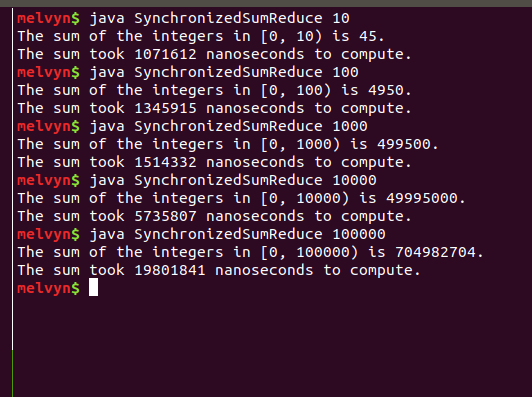
\includegraphics[width=0.5\textwidth]{Images/atomicOverflow.png}
  \caption{Creating a class that extends `Runnable'}
\end{figure}



\subsection{Exercise}
Change the above code to use an \textit{AtomicLong} instead of an
\textit{AtomicInteger}. Verify that you can sum from 0 to 99999.

The things you'll need to change are:
\begin{enumerate}
\item Change all \textit{AtomicInteger}s to \textit{AtomicLong}s
\item Change \textit{partialSum} to a \textit{long}
\item Change the parameter to \textit{updateTotal} to a \textit{long}
\end{enumerate}

\subsection{Last Note about Atomic Types}
There seems to have been some enhancements done around the release of Java 8.
Look at the docs:

Methods added for Java 8:

\url{https://docs.oracle.com/javase/8/docs/api/java/util/concurrent/atomic/AtomicLong.html}

\url{https://docs.oracle.com/javase/8/docs/api/java/util/concurrent/atomic/AtomicInteger.html}

Compared to Java 7:

\url{https://docs.oracle.com/javase/7/docs/api/java/util/concurrent/atomic/AtomicLong.html}

\url{https://docs.oracle.com/javase/7/docs/api/java/util/concurrent/atomic/AtomicInteger.html}

\subsection{If time to kill}
The overflow when we tried to sum 0 to 99999 in an integer was 7xxxxxxx. Using
knowledge of twos complement and binary addition, does that make sense?

4999950000 - 2147483648 = 2852466352
2852466352 - 2147483648= 704982704
\end{document}

